%\documentclass[UTF8]{book} % 使用book文档类型格式排版
\usepackage{ctex}  %加载包,因为我们在用中文写文档,所以必须加载这个包,否则不支持中文

%加入了一些针对XeTeX的改进并且加入了 \XeTeX 命令来输入漂亮的XeTeX logo
\usepackage{xltxtra}
%启用一些LaTeX中的功能
\usepackage{xunicode}

\usepackage{multicol}  %加载包
\usepackage{amsmath} % 调用公式宏包
\usepackage{amssymb} % 数学符号生成命令
\usepackage{array} % 数组和表格制作
\usepackage{booktabs} % 绘制水平表格线
\usepackage{calc} %四则运算
\usepackage{caption} % 插图和表格标题格式设置
\usepackage{fancyhdr} % 页眉页脚设置
\usepackage{graphicx} % 调用插图宏包
\usepackage{multicol} % 多栏排版
\usepackage{titlesec} % 章节标题格式设置

%%%% 目录样式 %%%%
\usepackage{titletoc}
\titlecontents{chapter}[1pt]{\vspace{.5\baselineskip}\bfseries}
    {{\thecontentslabel}\quad}{}
    {\hspace{.5em}\titlerule*[10pt]{$\cdot$}\contentspage}
\titlecontents{section}[2em]{\vspace{.25\baselineskip}\bfseries}
    {\thecontentslabel\quad}{}
    {\hspace{.5em}\titlerule*[10pt]{$\cdot$}\contentspage}

\usepackage{color}
\usepackage{xcolor} % 颜色处理
%\usepackage{indentfirst} % 自动首行缩进
%\setlength{\parindent}{2.22em} % 设置首行缩进的距离
% 设置超链接颜色
\usepackage[colorlinks=true,linkcolor=black,urlcolor=black,citecolor=black]{hyperref} % 根据章节标题生成PDF书签

%%%% 版面 %%%%
\usepackage[top=0.5in,bottom=0.5in,left=1.25in,right=0.8in]{geometry}
% 设置行距
\linespread{1}
\usepackage{lscape}
\usepackage{listings} %插入代码,代码页需要加入[fragile]
\usepackage{xeCJK}

%\usepackage[slantfont,boldfont]{xeCJK} % 允许斜体和粗体

%%%% fontspec 宏包 %%%%
\usepackage{fontspec}
% 指定字体
%\setmonofont[Mapping={}]{Monaco}	%英文引号之类的正常显示,相当于设置英文字体
%\setsansfont{Monaco} %设置英文字体 Monaco, Consolas,  Fantasque Sans Mono
%\setmainfont{Monaco} %设置英文字体
% \setCJKmainfont{方正兰亭黑简体}  %中文字体设置
% \setCJKsansfont{华康少女字体} %设置中文字体
% \setCJKmonofont{华康少女字体} %设置中文字体

%%%%%%%%%% 图形支持宏包 %%%%%%%%%%
\usepackage{graphicx}                % 嵌入png图像
\usepackage{color,xcolor}            % 支持彩色文本、底色、文本框等
%\usepackage{subfigure}
%\usepackage{epsfig}                 % 支持eps图像
%\usepackage{picinpar}               % 图表和文字混排宏包
%\usepackage[verbose]{wrapfig}       % 图表和文字混排宏包
%\usepackage{eso-pic}                % 向文档的部分页加n副图形, 可实现水印效果
%\usepackage{eepic}                  % 扩展的绘图支持
%\usepackage{curves}                 % 绘制复杂曲线
%\usepackage{texdraw}                % 增强的绘图工具
%\usepackage{treedoc}                % 树形图绘制
%\usepackage{pictex}                 % 可以画任意的图形
%\usepackage{hyperref}

%\setCJKmainfont{Kai}   % 设置缺省中文字体
%\setCJKmonofont{Hei}   % 设置等宽字体
%\setmainfont{Optima}   % 英文衬线字体
%\setmonofont{Monaco}   % 英文等宽字体
%\setsansfont{Trebuchet MS} % 英文无衬线字体

\makeatletter
\providecommand*\input@path{}
\newcommand\addinputpath[1]{
\expandafter\def\expandafter\input@path
\expandafter{\input@path{#1}}}
\addinputpath{body/}
\makeatother

\definecolor{keywordcolor}{rgb}{0.8,0.1,0.5}
\lstset{language=C++, %用于设置语言为C++
    numbers=left, %设置行号位置
    numberstyle=\tiny, %设置行号大小
    keywordstyle=\color{keywordcolor} \bfseries,
    identifierstyle=,
    basicstyle=\ttfamily,
    commentstyle=\color{blue} \textit, %注释颜色
    stringstyle=\ttfamily,
    showstringspaces=false,
    frame=shadowbox, %边框
    %frame = single,
    tabsize=2, %设置tab空格数
    showspaces=false, %不显示空格
    escapeinside=``, %逃逸字符(1左面的键),用于显示中文
    %breaklines, %自动折行
    captionpos=b
}
%\begin{document}

\chapter{数论}

\section{一些理论}

\subsection{大整数取模}

把大整数写成“从左向右”的形式:如:$1234 = ((1*10 + 2) * 10 + 3) * 10 + 4$. 然后根据$( n + m) \% p = ((n \% p) + (m \% p)) \% p$,每步取模。

\begin{lstlisting}
scanf("%s%d", &s, &p);
int len = strlen(s);
if(s[0] == '0' && len == 1){
    printf("divisible\n");
    continue;
}
if(p < 0) p = -p; //判断负数
int ans = 0, st = 0;
if(s[0] == '-') st = 1;
for(int i = st; i < len; i++){
    ans = (int)(((ll) ans * 10 + s[i] - '0') % p); //注意爆int
}
if(ans == 0) printf("divisible\n");
else printf("not divisible\n");
\end{lstlisting}

\subsection{哥德巴赫猜想($1+1$问题)}

大于$2$的所有偶数都可以表示为两个素数的之和,大于$5$的所有奇数均可以表示为三个素数之和。\\
陈景润证明了:所有大于$2$的偶数均是一个素数和只有两个素数因数的合数之和($1+2$问题),称为陈氏定理。

\subsection{费马小定理}
$p$是素数,且$a$  $!\equiv 0 $$(mod$ $ p)$,则:$a^{p - 1}  \equiv 1 (mod$ $p)$.

\subsection{素数定理}
$f(x) \approx \frac{x}{ln(x)}$ ($f(x) $为不超过$x$的素数的个数) \\
$10^{8}$级别的素数筛筛选出的素数个数约为$6 * 10^{6}$级别 \\
$10^7$级别的素数筛筛选出的素数个数约为$7 * 10^{5}$级别

\subsection{算数基本定理}

任何一个大于$1$的自然数$n$,若其不为素数则必可唯一的分解为有限个素数的乘积,即 $n = p_1^{a1} * p_2^{a2} * p_3^{a3} * ... * p_k^{ak}$,那么同时$n$的因子个数为$num = \prod (a_i + 1)(1 \leq i \leq k)$【$LightOJ\  1341$】。 \\

\subsection{$ax+by=c$的任意整数解}
$a,b,c$为任意整数,若$ax + by = c$的一组整数解为$(x_0, y_0)$,则它的任意整数解为$(x_0 + kb', y_0 - ka')$.其中$a'=\frac{a}{gcd(a,b)},b'=\frac{b}{gcd(a,b)}$,$k$取任意整数。 \\

证明:令$g = gcd(a, b)$.设另一组解为$(x_1, y_1)$,则$ax_0 + by_0 = ax_1 + by_1 (=c)$.移项:$a(x_1 - x_0) = b(y_0 - y_1)$.同除以$g$可得:$\frac{a} {g }* (x_1- x_0) = \frac{b}{g} * (y_0 - y_1)$.令$a' =\frac{ a }{g}, b' = \frac{b}{g}$。则$a'(x_1 - x_0) = b'(y_0 - y_1)$此时$a'$与$b'$互质.所以:$x_1 - x_0$一定是$b'$的整数倍,设倍数为$k$。则有:$x_1 - x_0 = kb', y_0 - y_1 = ka'$,可得:$x_1 = x_0 + kb', y_1 = y_0 - ka'$.结论加强:$a,b,c$为任意整数,$g=gcd(a,b)$,方程$ax + by = g$的一组解是$(x_0, y_0)$.则当$c$是$g$的倍数时,$ax+by=c$ 的一组解为$(\frac{x_0*c}{g}, \frac{y_0 * c}{g})$.当$c$不为$g$的倍数时$ax+by=c$无整数解。 \\

\subsection{$n$是$m$的倍数,$[1,n]$中和$m$互素数个数}
对于两个正整数$m$和$n$,如果$n$是$m$的倍数,那么$1\sim n$中与$m$互素的数的个数为$\frac{n}{m} * \phi(m)$.($\phi(m)$为小于等于$m$的且与$m$互素的数的个数)

\subsection{$p$为奇素数,$1\sim(p - 1)$ 模$p$的逆元对应全部$1\sim(p-1)$中的所有数,既是单射也是满射}
也就是$(1 + \frac{1}{2} + \frac{1}{3} + ... + \frac{1}{(p -1)}) \ mod (\ p) = ( 1 + 2 + ... + (p - 1))\ mod(\ p)$.

\subsection{调和级数求和}
令$h[n]$表示$n$级调和级数的和,即:$h[n] = \frac{1}{1} + \frac{1}{2} + \frac{1}{3} + \frac{1}{4} +...+ \frac{1}{n}$.则当$n > 10^{6}$ 时可以用公式:
$$h[n]=(log(n * 1.0) + \frac{log(n + 1.0)}{2.0} + \frac{1.0}{(6.0 * n * (n + 1))} -\frac{1.0}{(30.0 * n * n * (n + 1) * (n + 1))} + r$$
其中$r$ 为欧拉常数:$r= 0.57721566490153286060651209008240243104215933593992$。上述公式误差不超过$10^{-8}$.

\subsection{如果$gcd(a,m)=1$,那么$gcd(a+k*m,m)=1,k\in Z$}
\underline{【$POJ\ 2773$】}

证明:只需要证明$gcd(a+m, m)=1$.令$d=gcd(a+m,m)$,设$a+m=d*p_1,m=d*p_2且p_1>p_2,$,移项可得:$a=d*(p_1-p_2)$,如果$d!=1$,那么$gcd(a,m)!=1$,与原条件不符,故$gcd(a,m)=1$,同理可证$gcd(a+k*m,m)=1,k\in Z$.

\subsection{指数降幂公式}
$$A^{x}\ \% \ p=A^{x\%\phi(p)+\phi(p)}\  \% \ p\ (x\geq \phi(p))$$
其中$\phi(p)$是$p$的欧拉函数值

\clearpage
\section{素数筛}

\begin{lstlisting}
void GetPrime(int n ) //获得 n 以内的所有质数
{
    prime_cnt = 0;
    int m = sqrt(n + 0.5);
    memset(vis, 0, sizeof(vis));
    for(int i = 2; i <= m; i++){
          if(vis[i] == 0){
              prime[prime_cnt++] = i;
              for(int j = i * i; j < n; j+= i){
                   vis[j] = 1;
              }
          }
    }
}

//线性时间素数筛:利用每个合数必有一个最小素因子,每个合数仅被它的最小素因子筛去
//代码核心:if(i % prime[j] == 0) break;
void GetPrime()
{
    prime_cnt = 0;
    memset(vis, 0, sizeof(vis));
    for(int i = 2; i < MAX_N; i++){
        if(vis[i] == 0) { prime[prime_cnt++] = i; }
        for(int j = 0; j < prime_cnt && i * prime[j] < MAX_N; j++){
            vis[i * prime[j]] = 1;
            //将所有合数标记, prime[j] 是 i * prime[j] 的最小素因子
            if(i % prime[j] == 0) break;
        }
    }
}
\end{lstlisting}

\subsection{区间素数筛}
\begin{lstlisting}
const int MAX_N = 100010; // 最大区间长度

int prime_cnt;
int prime_list[MAX_N];
bool prime[MAX_N]; //prime[i] = true:i + L 是素数

void SegmentPrime(int L, int R)
{
    int len = R - L + 1; // 区间长度
    for(int i = 0; i < len; i++) prime[i] = true; // 初始全部为素数
    int st = 0;
    if(L % 2) st++; // L 是奇数
    for(int i = st; i < len; i += 2) { prime[i] = false; }
    // 相当于 i + L 是合数,把 [L, R] 的偶数都筛掉
    int m = (int)sqrt(R + 0.5);
    for(int i = 3; i <= m; i += 2){ // 用 [3, m] 之间的数筛掉 [L, R] 之间的合数
        if(i > L && prime[i - L] == false) { continue; }
        // i 是 [L, R] 区间内的合数,此时 [L, R] 区间中中以 i 为基准的合数已经被筛掉了
        int j = (L / i) * i; // 此时 j 是 i 的倍数中最接近 L (小于等于 L )的数
        if(j < L) j += i; // j >= L
        if(j == i) j += i;
        // 如果 j>=L 且 j==i 且 i 为素数,则相当于 [L, R] 中的 i 也为素数,所以要 j+=i
        j -= L; // 把 j 调整为 [0, len) 之间
        for(; j < len; j += i) {
            prime[j] = false;
        }
    }
    if(L == 1) prime[0] = false;
    if(L <= 2) prime[2 - L] = true;   // 特别注意 2 的情况!
    prime_cnt = 0;
    for(int i = 0; i < len; i++){
        if(prime[i]) prime_list[prime_cnt++] = i + L;
    }
}
\end{lstlisting}

\section{约数筛}
定义$e[i]$表示$i$的最小质因子的幂次,$div\_num[i]$表示$i$的约数个数。 \\
考虑在素数筛的过程中,$e[i]$的更新:
\begin{itemize}
\item $i$为质数:$e[i]$
\item $i \% prime[j]==0:e[i*prime[j]]=e[i]+1$
\item $i \% prime[j]!=0:e[i*prime[j]]=1$
\end{itemize}
$div\_num[i]$的更新:
\begin{itemize}
\item $i$为质数:$div\_num[i]=1$
\item $i \% prime[j]==0:div\_num[i*prime[j]]=\frac{div\_num[i]}{e[i]+1}*(e[i]+2)$
\item $i \% prime[j]!=0:div\_num[i*prime[j]]=div\_num[i]*div\_num[prime[j]]\quad $(积性函数的性质)
\end{itemize}

\begin{lstlisting}
const int MAX_N = 1000010;

int prime_cnt = 0;
int prime[MAX_N], e[MAX_N], div_num[MAX_N], vis[MAX_N];

void Sieve() {
	e[1] =   0, div_num[1] = 1;
	for (int i = 2; i < MAX_N; ++i) {
		if (vis[i] == 0) {
			prime[prime_cnt++] = i;
			e[i] = 1;
			div_num[i] = 2;
		}
		for (int j = 0; j < prime_cnt && i * prime[j] < MAX_N; ++j) {
			int now = i * prime[j];
			vis[now] = 1;
			if (i % prime[j] == 0) {
				e[now] = e[i] + 1;
				div_num[now] = div_num[i] / (e[i] + 1) * (e[i] + 2);
				break;
			} else {
				e[now] = 1;
				div_num[now] = div_num[i] * div_num[prime[j]];
			}
		}
	}
}
\end{lstlisting}

\subsection{51nod 1586}
有三个下标从1到$n$的数组$a,b,c$。$a$数组初始全为0。
$$
b[i]=\sum_{j|i}{}a[j]\qquad c[i]=\sum_{j|i}{}b[j]
$$
需要进行下列操作:
\begin{itemize}
\item $1\ x\ y$ :将$a[x]$加上$y\quad (x\in [1,n],y\in [1, 10^6])$
\item $2\ x$ :询问当前$c[x]\quad (x\in [1,n])$的值
\end{itemize}
对每次查询输出答案。 \\

每次$a[x]$添加$y$,那么$b[r]_{i|r}$都会添加$y$,而$c[s]_{i|s}$添加的数字是:$div\_num[\frac{s}{i}]*x$。
\begin{lstlisting}
int n, Q;
ll C[MAX_N];

int main() {
	Sieve();
	scanf("%d%d", &n, &Q);
	while (Q--) {
		int type, x, y;
		scanf("%d", &type);
		if (type == 1) {
			scanf("%d%d", &x, &y);
			for (int i = x; i <= n; i += x) {
				C[i] += 1ll * div_num[i / x] * y;
			}
		} else {
			scanf("%d", &x);
			printf("%lld\n", C[x]);
		}
	}
	return 0;
}
\end{lstlisting}

\section{分解质因数}

\begin{lstlisting}
void factor(int x)
{ // factot: 存质因数, factor_cnt[i] :存 factor[i] 的指数, factor_num :质因数的个数
    GetPrime();
    factor_num = 0;
    memset(factor_cnt, 0, sizeof(factor_cnt));
    for(int i = 0; i < prime_cnt && prime[i] * prime[i] <= x; i++){
          if(x % prime[i] == 0){
               int tmp  = 0;
              while(x % prime[i] == 0){
                   x /= prime[i];
                   tmp ++;
              }
              factor[factor_num] = prime[i];
              factor_cnt[factor_num++] = tmp;
          }
    }
}
\end{lstlisting}

\subsection{给定$n$求满足$a^p = n$的最大$p$}

\underline{【LightOJ  1220】} \\

需要考虑$n$的正负。对于正数$n$只要对$n$进行质因子分解,然后在所有质因子的幂中找$gcd$即可。 \\
对于负整数$n$需要考虑质因子的幂为偶数的情况,因为得到的质因子实际上是它的相反数,如果是偶数次幂的话 得到的是正数,所以需要将偶数次幂除以$2$找到把幂变为奇数。例如对于$-16$,分解质因子得到$2$和幂次$4$.需要将$\frac{4}{2}$得$2$,再除以$2$得$1$,所以答案就是$1$. 然而对于$n = -32$来说,就不用了,因为得到$2$的幂次是$5$是个奇数,答案就是$5$. \\

\subsection{求满足$lcm(i, j) = n(1\leq i \leq j \leq n\leq 10^{14})$的$(i, j)$对数}

\underline{【LightOJ  1236】}\\

假设$n$质因子分解为:$n = p_1^{e_1} * p_2^{e_2} * p_3^{e_3} * ... * p_k^{e_k}$。对于任意${p_i}$的幂${e_i}$,当对$i,j$进行质因数分解后, 相应的到的$p_i$的幂为$a_i$和$b_i$,那么一定满足$max(a_i, b_i)=e_i$. 如果$a_i = e_i$,那么$b_i$可以取$[0, e_i]$,共$e_i+1$ 种, 如果$a_i < e_i$,那么$b_i$只取$e_i$,这时$a_i$可以取$[0, e_i)$,共$e_i$种。 合起来一共是$2*e_i+1$种。所以对每个质因子这样考虑的话可以得到:$ans = ∏(2*e_i+1)$. 但是要考虑到$i\leq j $,所以$ans = \frac{ans}{2}$, 但是上面的考虑在所有的$p_i$当中$a_i = e_i$同时$b_i = e_i$只考虑了一次,也就是$i=j=n$只考虑了一次。所以还要$ans = ans + 1$.

\section{逆元}

\subsection{介绍}
对于正整数$a,p$满足$ax \equiv 1 (\% \ p)$的最小正整数$x$称为$a$的逆元。 \\
乘法逆元的存在条件是:$gcd(a,p)=1$。 \\
$\equiv$:同余符号。$a \equiv b (mod \ n)$的含义是"$a$和$b$关于模$n$同余",即$a\  mod\ n = b\ mod\ n$,其充要条件是:$a - b$ 是$n$ 的整数倍.当$gcd(a, n) = 1$时,该方程有唯一解,否则该方程无解。  \\
特例: \\
$1$:当$p$是素数且$a\ != 0 (mod\ p)$时由费马小定理可得:$x \equiv a ^{(p - 2)} (mod\ p)$. \\
$2$:已知$b\ |\ a$,则$(\frac{a}{b})\ mod\ m=\frac{a\  mod\  (mb)} {b}$。这个式子通常用于模数和分母不互素的情况,这样就不能用费马小定理和扩展欧几里德求解,必须将模数扩大为$m*b$,最后答案除以$b$。 \\
证明:假设$\frac{a}{b}\ mod (m) = x$, \\
即:$\frac{a}{b} = k * m + x (x < m)$ \\
$-->a = k * b * m + b * x$ \\
$-->a\ mod\ (bm) = bx$ \\
$-->\frac{a\ mod\ (bm)}{b} = x$ \\
$-->\frac{a}{b}\ mod(m) =\frac{a\ mod\  (bm)}{b}\ = \ x$ \\

\subsection{模素数逆元连乘}

如果有的题目需要用到$1\sim n$模$M$的所有逆元($M$为奇质数),如果用快速幂求解时间复杂度为$O(M*log(M))$.实际上有$O(M)$的算法,递推式如下: \\
$$inv[i] = (M - \frac{M}{i} ) * inv[M\  \%\  i] \% M$$
推导过程如下: \\
设$t = \frac{M} {i},k = M \% i --> t * i + k = 0\ (mod\ M) -->-t * i = k\ (mod\ M)$.两边同时除以$i * k$得:$--> -t * inv[k] = inv[i](mod\  M)$.再把$t$和$k$替换掉最终得到:
$$inv[i] = (M - \frac{M} {i}) * inv[M\  \%\  i] \% \ M$$
初始化$inv[1] = 1$.这样就可以通过递推法求出$1\sim n$模$M$的所有逆元了。

\begin{lstlisting}
ll inv(ll a, ll p) // 利用 inv[a] = (p - p / a) * inv[p % a] % p 求逆元
{ // 需要保证 a < p 且 gcd(a, p) = 1
	if(a == 1) return 1;
	return inv(p % a, p) * (p - p / a) % p;
}
\end{lstlisting}

\section{欧拉函数}

\subsection{介绍}

定义:$\phi[n]$:小于等于$n$且与其互素的正整数的个数 \\
欧拉定理:$a^{\phi(n)} \equiv 1(mod\ n)\ (gcd(a,\ n) = 1)$ \\
特例是费马小定理。利用这个定理求模意义下的乘法逆元:$a^{-1}\equiv a^{\phi(n)-1}(mod\ n)$ \\
性质:
\begin{itemize}
\item $\phi(1) = 1$
\item $\phi(N) = N· \prod \frac{p-1}{p}$ ($p$为$N$的所有素因数)
\item $\phi(p^k)= p^k−p^{k−1} = (p−1)·p^{k−1},$其中$p$为素数
\item $\phi(m * n) = \phi(m)·\phi(n)$,其中 $gcd(m,n) = 1$
\item $\sum_{d|n}{}\phi(d) = n$
\item 当$p$为素数时:$$\phi(t * p)=\left\{
 \begin{array}{rcl}
 p*\phi(t)& & t \% p =0 \\
 (p-1)*\phi(t)& & t \% p != 0\\
 \end{array}\right.$$
\item 当$n>1$时,$1...n$中与$n$互质的整数和是$\frac{n\phi(n)}{2}$
\item 当$n \geq 3$时,$\phi[n]$是偶数
\item 两相邻质数之间合数的欧拉函数值小于较小的素数,所以对于一个数$x$要找到最小的$t$使得$t$的欧拉函数值$\phi[t] \geq x$ 则$t$必然是大于$x$的第一个素数。
\item 若$(n\ \%\ p\ ==\ 0\ \&\&\ \frac{n}{p}\ \%\ p\ ==\ 0)$则有:$\phi (n)=\phi (\frac{n}{p})*p$;
\item 若$(n\ \%\ p\ ==\ 0\ \&\&\ \frac{n}{p}\ \%\ p\ !=\ \ 0)$则有:$\phi (n)=\phi (\frac{n}{p})*(p-1)$;
\end{itemize}
其中$p$是$n$的质因数

\subsection{求单个数的欧拉函数}
求欧拉函数:先令$\phi[i] = i$,根据性质$2$,遍历所有素数$p$,令$\phi[kp] = \frac{\phi[kp]}{ p }* (p − 1)$
\begin{lstlisting}
// 任何一个大于 1 的自然数 n ,若其不为素数则必可唯一的分解为有限个素数的乘积
int Euler(int n)
{
    int ans = 1;
    for(int i = 2; i * i <= n; i++){
        if(n % i == 0){
            n /= i;
            ans *= (i - 1);
            while(n % i == 0){
                n /= i;
                ans *= i;
            }
        }
    }
    if(n > 1) ans *= (n -1);
    return ans;
}
\end{lstlisting}

\begin{lstlisting}
int Euler(int n)
{
    int res = n, a = n;
    for(int i = 2; i * i <= a; i++){
        if(a % i == 0){
            res = res / i * (i - 1); // 先进行除法防止数据溢出
            while(a % i ==0) a /= i;
        }
    }
    if(a > 1) res = res / a * (a - 1);
    return res;
}
\end{lstlisting}

\subsection{欧拉筛}
\begin{lstlisting}
void GetPhi() // 埃氏筛
{
    phi[1] = 1;
    for(int i = 2; i < MAX_N; i++){
        if(phi[i] == 0){
            for(int j = i; j < MAX_N; j += i){
                if(!phi[j]) phi[j] = j;
                phi[j] = phi[j] / i * (i - 1);
            }
        }
    }
}
\end{lstlisting}

\begin{lstlisting}
bitset<MAX_N> bs;
int prime_cnt, prime[MAX_N], phi[MAX_N];
void GetPhi() // 欧拉筛,同时获得素数表和欧拉表
{
	prime_cnt = 0;
	bs.set();
	for(int i = 2; i < MAX_N; ++i ) {
		if(bs[i] == 1) {
			prime[prime_cnt++] = i;
			phi[i] = i - 1;
		}
		for(int j = 0; j < prime_cnt && i * prime[j] < MAX_N; ++ j ) {
			bs[i * prime[j]] = 0;
			if(i % prime[j]) {
				phi[i * prime[j]] = (prime[j] - 1) * phi[i];
			}else {
				phi[i * prime[j]] = prime[j] * phi[i];
				break;
			}
		}
	}
}
\end{lstlisting}

\underline {[UVA 11428  GCD - Extreme (II):给定$n$求:$G= \sum_{i=1}^{i<N} \sum_{j=i+1}^{j\leq N}GCD(i, j) (n \leq 4000000)$} \\

令$sum[n]$为题式中答案。考虑递推$sum[n] = sum [n - 1] + gcd(1, n) + gcd(2, n) + gcd(3, n) + ... + gcd(n - 1, n)$ 。令$f[n] = gcd(1, n) + gcd(2, n) + gcd(3, n) + ... + gcd(n - 1, n)$. 设满足$gcd(x, n) = t ...①$的$x(x < n)$的个数有$h[t]$个,显然$x, t$均是$n$的约数,又因为不包含$gcd(n, n)$,所以$t < n$。 将等式$①$两边同除以$t$可得:$gcd(\frac{x}{t}, \frac{n}{t}) = 1$.所以$h[t] = \phi[\frac{n}{t}]$. 那么枚举$n$的约数可以得到:$f[n]=\sum_{}(t*\phi[\frac{n}{t}])$($t$为$n$的所有约数) $- n$(相当于去掉$gcd(n, n)$) 需要预处理$f[n]$然后对于每个$n$有:$sum[i] = sum[i - 1] + f[i]$,$sum[1] = 0$;递推即可。
\begin{lstlisting}
typedef long long ll;
const int MAX_N = 4000010;

int n;
ll phi[MAX_N], f[MAX_N], sum[MAX_N];

void init()
{
    GetPhi();
    memset(f, 0, sizeof(f));
    for(int i = 1; i < MAX_N; i++){
        for(int j = i; j < MAX_N; j += i){
            f[j] += i * phi[j / i];
        }
    }
}

int main()
{
    init();
    while(~scanf("%d", &n) && n){
        sum[1] = 0;
        for(int i = 2; i <= n; i++){
            sum[i] = sum[i - 1] + f[i] - i;
        }
        printf("%lld\n", sum[n]);
    }
    return 0;
}
\end{lstlisting}

\section{扩展欧几里德}

\subsection{裴蜀定理}
$ax + by = gcd(a, b)必有一组解(x,y)$. \\

求解过程:因为a$x + by = gcd(a, b)$且$gcd(a, b) = gcd(b, a \% b)$。那么有:$bx + (a \% b)y = gcd(b, a \% b)$,即有:$ bx + (a \% b)y = ax + by$.所以:$bx' + (a - \frac{a}{b} * b)y' = ax + by。$移项$:ay' + b(x' -\frac{ a}{b} * y') = ax + by$.得到: $x = y', y = (x' - \frac{a} {b} * y')$,也就是$x' = y - \frac{a} {b} * x, y' = x$.所以可以使用递归求解。

\begin{lstlisting}
//需保证系数 a, b 应同为正数,但是求解出来的 x, y 可正可负
int ex_gcd(int a, int b, int& x,int& y)
{
    if(b == 0) {
          x = 1, y = 0;
          return a;
    }
    int r = ex_gcd(b, a % b, y, x);
    y -= a / b * x;
    return r;
}
\end{lstlisting}
\underline{解释1:$y -= \frac{a}{b} * x$} \\

由前面的推导可知: $x' = y -\frac{a}{b} * x, y' = x$,其中$x,y$是真正解,$x',y'$是递归调用时的下一层的解。所以需要将上一层的$x$ 传递给下一层的$y'$,另一方面因为$x$和$y$是未知的所以不能直接将上一层的$y - a / b * x$ 传递给下一层的$x'$,但是可以先传递$y$, 相当于人为的增加了$\frac{a}{b} * x$,所以当计算出真正的$x,y$时需要减去$\frac{a}{ b }*x$.
\underline{解释2:$ x = 1, y = 0$} \\

递归的最后一层的方程式的是:$gcd(a,b) * x + 0 * y = gcd(a, b)$.要使这个式子恒成立,显然需要$x = 1。$递归的倒数第二层的方程式是:$k * gcd(a, b) * x' + gcd(a, b) * y' = gcd(a, b)$.其中$k$为任意整数。约掉$gcd(a, b)$可得:$k * x' + y' = 1.$此式要恒成立显然$x' = 0, y' = 1$。 又因为此式中的$x' = y, y' = x - \frac{a} {b} * y$.所以$y = 0$.当然这时$y' = x - \frac{a}{b} * y = 1 -\frac{a}{b} * 0 = 1$.正好也是符合的。

\subsection{求解逆元$ax \equiv 1 (mod\  n)$的最小非负数解}
先求解:$ax + ny = gcd(a, n)$.如果$gcd(a, n) = 1,$则$ans = (x \% n + n) \% n$.否则无解。所以题目中经常是n为一个很大的素数,这样保证了$gcd(a, n) = 1.$ \\
这里得到的是最小非负数解$x$ ,如果要求$x$为正数还要在$return$时特判:$if(x == 0) x = n;$

\begin{lstlisting}
int Inv(int a, int n) // Module Inverse 模逆元
{
    int d, x, y;
    d = ex_gcd(a, n, x, y);
    if(d == 1) return (x % n + n) % n;
    // a 和 n 的最小公倍数是 1 ,此时解存在
    else return -1; //no solution
}
\end{lstlisting}

\subsection{求所有解中$C = |x| + |y|$最小值}

假设基础解为$(x_0, y_0)$,那么通解可以表示为:$x = x_0 + k * b, y = y_0 - k * a(k ∈ Z)$。 如果令$x = 0$得:$k = -\frac{x_0}{b}...①$,令$y = 0$ 得:$k = \frac{y_0}{a}...②$当两者同时满足并根据分数的性质:$\frac{a}{b} =\frac{c}{d} = \frac{(a + c)}{(b + d) }$可得:$ k = \frac{(y_0 - x_0)}{(b + a)}$,但是考虑到这个数的真实值可能为浮点数,需要左右考虑。

\begin{lstlisting}
ll solve(ll a, ll b, ll t) // 方程为 a * x + b * y = t
{
    ll x, y, d, res;
    d = ex_gcd(a, b, x, y);
    if(t % d) return -1;
    a /= d, b /= d, t /= d;
    x *= t, y *= t; //此时 x, y 为基础解
    res = (ll)1e18;
    ll tmpx, tmpy, c = (y - x) / (a + b);
    for(int i = c - 1; i <= c + 1; i++){ //左右考虑
        tmpx = x + i * b, tmpy = y - i * a;
        res = min(res, abs(tmpx) + abs(tmpy));
    }
    return res;
}
\end{lstlisting}

\subsection{求最小非负整数解$x$和此时的$y$}
\begin{lstlisting}
ll extra = 0;
if(x < 0) extra = 1;
ll t = x / b - extra;
printf("%lld %lld\n", x - t * b, y + t * a);
\end{lstlisting}

\section{模线性方程组}
\underline{输入正整数$a,b,n$,解方程$ax≡b(mod\ n).a,b,n\leq 10^9$}

把$ax\equiv b(mod n)$转化为$ax - ny = b$,当$d = gcd(a, n)$不是$b$的约数时无解,否则两边同时除以$d$,得到$a'x - n'y = b'$,即$ax' \equiv b'(mod n')$(这里$a' =\frac{a}{d},b' =\frac{b} {d} ,n'=\frac{n}{d}$).此时$a'$和$n'$已经互素,因此只需要左乘$a'$在模$n'$下的逆,则解为$x≡(a')^{-1}* b' (mod\  n')$,这个解是模$n'$剩余系中的一个元素。还需要把解表示成模$n$剩余系中的元素。 \\
令$p = (a')^{-1} * b'$,上述解相当于$x = p, p+n', p+2*n',p+3*n'...$。对于模$n$来说,假定$p+i*n'$和$p+j*n'$同余,则$(p+i*n') - (p+j*n') = (i-j)*n'是n$的倍数。因此$(i-j)$必须是$d$的倍数。也就是说,在模$n$剩余系下,$ax\equiv b(mod n)$恰好有$d$个解,为$p,p+n',p+2*n',...,p+(d-1)*n'$.

\subsection{利用扩展欧几里德求解模线性同余方程 $ax\equiv b(mod n)$}
如果$gcd(a,b)$不能整除$c$则$ax+by=c$无整数解。对于$ax\equiv b(mod n)(n>0)$,上式等价于二元一次方程$ax-ny=b$
\begin{lstlisting}
bool ModularLinearEquation(int a, int b, int n)
{
    int x, y, x0;
    int d = ex_gcd(a, n, x, y); //d = gcd(a,n)
    if(b % d) return false; // d 不能整除b
    x0 = x * (b / d) % n; //basic solution
    for(int i = 1;i <= d; i++){
        printf("%d\n", (x0 + i * (n / d) % n));
    }
    return true;
}
\end{lstlisting}

\underline{[SGU 106]给出$a,b,c,x_1,x_2,y_1,y_2$求满足$ax + by + c = 0$且$x\in[x_1,x_2]$,$ y\in[y_1,y_2]$的$x,y$有多少组。} \\

 相当于问在直线$ax + by + c = 0$上有多少整点$(x,y)$满足$x\in[x_1,x_2]$,$ y\in[y_1,y_2]$.扩展欧几里德的应用。需要特别注意$a=0,b=0,c=0$ 的特判。
\begin{lstlisting}
typedef long long ll;
double eps = 1e-8;

ll a, b, c, x1, yy1, x2, y2, ans;

ll ex_gcd(ll n, ll m, ll& x, ll& y) // 返回值是 gcd(a, b)
{
    if(m == 0){
        x = 1, y = 0;
        return n;
    }
    ll d = ex_gcd(m, n % m, y, x);
    y -= n / m * x;
    return d;
}

void ModularLinearEquation() // 模线性方程组
{
    ll x, y, x0, y0;
    ll d = ex_gcd(a, b, x, y);// 求解方程ax+by=gcd(a, b)
    if(c % d) {
        printf("0\n");
        return ;
    }
    // 此时的 x, y 是方程 ax + by = gcd(a, b) 的一组基础解
    a /= d, b /= d, c /= d;
    x0 = x * c, y0 = y * c; // x0, y0 是 ax + by = c 的一组基础解
    // a * x + b * y = c 通解满足: a * (x0 + k * b) + b * (y0 - k * a) = c
    //所以: x' = x0 + k * b ...①, y' = y0 - k * a ...②, k ∈ Z
    //先求出满足 1:x1 <= x0 + k * b <= x2 的 k 的范围 [l1, r1]
    //再求出满足 2:yy1 <= y0 - k * a <= y2 的 k 的范围 [l2, r2] 两者取交集即可
    //l1 = ceil((x1 - x0)/b),r1 = floor((x2 - x0)/b)
    //l2 = ceil((y0 - y2)/a), r2 = floor((y0 - yy1)/a)
    ll l1 = (ll)ceil((double)(x1 - x0) / b);
    ll r1 = (ll)floor((double)(x2 - x0) / b);
    ll l2 = (ll)ceil((double)(y0 - y2) / a);
    ll r2 = (ll)floor((double)(y0 - yy1) / a);
    ll l = max(l1, l2), r = min(r1, r2);
    ans = (r - l + 1 < 0) ? 0 : (r - l + 1);
    printf("%lld\n", ans);
    return ;
}

int main()
{
    while(~scanf("%lld%lld%lld", &a, &b, &c)){
        scanf("%lld%lld%lld%lld", &x1, &x2, &yy1, &y2);
        int flag = 0;
        c = -c; // 移项,得到方程a * x + b * y = -c
        // 下面将方程的所有系数 a, b, c 变为非负数
        if(c < 0){
            c = -c , a = -a, b = -b;
        }
        if(a < 0){
// 需要将 a 取相反数,相当于把 x 也取了相反数,所以需要将 [x1, x2] 的范围变为[-x2, -x1]
            ll tmpx1 = x1, tmpx2 = x2;
            x1 = -tmpx2, x2 = - tmpx1;
            a = -a;
        }
        if(b < 0){ // 同理
            ll tmpyy1 = yy1, tmpy2 = y2;
            yy1 = -tmpy2, y2 = -tmpyy1;
            b = -b;
        }

        if(a == 0 && b == 0) { //0 * x + 0 * y = c
            flag = 1;
            if(c == 0) ans = (x2 - x1 + 1) * (y2 - yy1 + 1);
            else ans = 0;
        }else if(a == 0){  // b != 0
            flag = 1;
            if(c % b == 0){ // 0 * x + b * y = c --> b * y = c
                ll tmpy = c / b;
                if(yy1 <= tmpy && tmpy <= y2) ans = x2 - x1 + 1;
                else ans = 0;
            }else ans = 0;
        }else if(b == 0) { //a != 0
            flag = 1;
            if(c % a == 0) { // a * x + 0 * y = c --> a * x = c
                ll tmpx = c / a;
                if(x1 <= tmpx && tmpx <= x2) ans = y2 - yy1 + 1;
                else ans = 0;
            }else ans = 0;
        }
        // 以上处理完了 a = 0 或者 b = 0 的所有特例
        if(flag)  printf("%lld\n", ans);
        else ModularLinearEquation();
    }
    return 0;
}
\end{lstlisting}

\section{中国剩余定理}
\underline{给定整数$n$和$n$个整数$a[i],m[i]$,求满足方程$ x \equiv a[i] (mod\  m[i])(0\leq i<n)$的最小正整数解。} \\

例如求解:满足$n = 3, a[0] = 2, m[0] = 3, a[1] = 3, m[1] = 5, a[2] = 2, m[2] = 7$.即: \\
$n \% 3 = 2 --> 5 * 7 * a \% 3 = 1 --> a = 2,a[0] = 2 \therefore a = 4 $得$:5 * 7 * 4$ \\
$n \% 5 = 3 --> 3 * 7 * b \% 5 = 1 --> b = 1,a[1] = 3 \therefore b = 3 $得$:3 * 7 * 3$ \\
$n \% 7 = 2 --> 3 * 5 * c \% 7 = 1 --> c = 1,a[2] = 2 \therefore c = 2 $得$:3 * 5 * 2$ \\
累加得: $5 * 7 * 4 + 3 * 7 * 3 + 3 * 5 * 2 = 233$ \\
取余得: $233 \% (3 * 5 * 7)= 23$, 所以最终答案就是 $23$

\subsection{模数互素}
\begin{lstlisting}
//前提条件: m[i] > 0 ,且 m[i] 中任意两数互质
ll CRT(ll a[], ll m[], ll n)
{ // Chinese Remainder Theorem
    ll M = 1, ans = 0;
    for(int i = 0; i < n; i++) { M *= m[i]; }
    for(int i = 0; i < n; i++){
        ll x, y, e;
        e = M / m[i];
        ex_gcd(e, m[i], x, y);
        ans = (ans + e * x % M * a[i] % M) % M;
    }
    return (ans + M) % M; //最小正整数解
}
\end{lstlisting}
\subsection{模数不互素}
当m[i]不满足两两互素时,假设$x \equiv a1(mod\ m1)...(1), x \equiv a2(mod\  m2)...(2).$ \\
令$d = gcd(m1, m2)$.由$(1)(2)$得:$x = a1 + m1 * k1, x = a2 + m2 * k2$.合并可得:$m1 * k1 = (a2 - a1) + m2 * k2$ \\
两边同除以$d$得:$m1/d * k1 = (a2 - a1) / d + m2 / d * k2$. \\
也就是: $m1 * k1 / d ≡ (a2 - a1) / d (mod\  m2/d)$. \\
也就是: $m1 * k1 = (a2 - a1) (mod\  m2)$. \\
易知$k1$有多个解,假设$k'$为$k1$的最小非负整数解则:$k1 \equiv k' (mod\  m2/d)$ \\
即:$k1 = k' + (m2 / d) * C$($C$为某一整数).将其带入$x = a1 + m1 * k1$ \\
可得:  $x = a1 + m1 * (k' + m2 / d * C)$ \\
也就是:$x = a1 + m1 * k' + m1 * m2 / d * C$。 \\
也就是: $x = (a1 + m1 * k') (mod\  m1 * m2 / d)$ \\
也就是: $x = (a1 + m1 * k') (mod\  lcm(m1, m2))....(3)$; \\
那么求解出$k'$后,就可以将方程(1)(2)合并为一个方程(3)了,依次迭代就能出解了。 \\
\underline{[HDU 1573 X问题]:求解在$(0, N]$区间满足 $x \equiv a[i](mod\  m[i])$($0\leq i < M)$的$x$的个数。} \\

利用中国剩余定理求解出最小非负整数解$a0$(如果有解)和解的周期$m0$,假设解的个数为$k$个 则:$a0 + k * m0 <= N --> k <= (N - a0) / m0,(N >= a0)$。 当$a0 = 0$时解的个数是$(N - a0) / m0$. 当$a0 > 0$时解的个数是$(N - a0) / m0 + 1$.

\begin{lstlisting}
typedef long long ll;
const int MAX_N = 15;

int T, M;
ll N, a0, m0, a[MAX_N], m[MAX_N];

ll ex_gcd(ll aa, ll bb, ll& xx, ll& yy)
{
    if(bb == 0) {
        xx = 1, yy = 0;
        return aa;
    }
    ll dd = ex_gcd(bb, aa % bb, yy, xx);
    yy -= aa / bb * xx;
    return dd;
}

//求解: m0 * x = (aa - a0) (mod mm)
bool ModularLinearEquation(ll& m0, ll& a0, ll mm, ll aa)
{
    ll x, y, d;
    d = ex_gcd(m0, mm, x, y);
    if(labs(aa - a0) % d != 0) return false;
    mm /= d;
    x = x * (aa - a0) / d % mm;
    a0 += x * m0;
    m0 *= mm;
    a0 = (a0 % m0 + m0) % m0;
    return true;
}

bool CRT(ll& m0, ll&a0)
{
    bool flag = true;
    m0 = 1, a0 = 0; //任意数 mod m0 = a0 恒成立
    for(int i = 0; i < M; i++){
        if(ModularLinearEquation(m0, a0, m[i], a[i]) == false){
            flag = false;
            break;
        }
    }
    return flag;
}

int main()
{
    scanf("%d", &T);
    while(T--){
        scanf("%lld%d", &N, &M);
        for(int i = 0; i < M; i++){
            scanf("%lld", &m[i]);
        }
        for(int i = 0; i < M; i++){
            scanf("%lld", &a[i]);
        }
        if(CRT(m0, a0) == false || N < a0) printf("0\n");
        else {
            //printf("a0 = %lld m0 = %lld\n", a0, m0);
            printf("%lld\n", (N - a0) / m0 + (a0 == 0 ? 0 : 1));
        }
    }
    return 0;
}
\end{lstlisting}

\section{法雷级数}

\subsection{介绍}
真分数:若$p,q$是正整数,$0 < \frac{p}{q} < 1$,则称$\frac{p}{q}$为真分数。 \\
定理:若$\frac{a}{d},\frac{c}{d}$是最简真分数(也可以是$\frac{0}{1},\frac{1}{1}$),且$\frac{a}{b} < \frac{c}{d}$则有: \\
\begin{itemize}
  \item 数$\frac{a + c} {b + d}$是一个最简真分数
  \item $\frac{a}{b} < \frac{a + c}{b + d} < \frac{c}{d}$
\end{itemize}

\subsection{$n$级法雷数列}
对于任意给定的自然数$n$,将分母小于等于$n$的不可约的真分数按升序排列,并且在第一个分数之前加上$\frac{0}{1}$,在最后一个分数之后加上$\frac{1}{1}$,这个序列称为$n$级法雷数列,用$F_n$表示。例如:$F_5:\frac{0}{1}, \frac{1}{5}, \frac{1}{4}, \frac{1}{3}, \frac{2}{5}, \frac{1}{2}, \frac{3}{5}, \frac{2}{3}, \frac{3}{4}, \frac{4}{5}, \frac{1}{1}$.

\subsection{法雷数列的构造}

应用上面的定理,如果$\frac{a}{b}和\frac{c}{d}$是一个法雷数列,则在它们中间可以插入$\frac{(a+c)}{(b+d)}$,这样一直二分构造,直到不能构造为止(分母大于$n$).例如$F_5$的构造: \\
$step1: $在$\frac{0}{1}$和$\frac{1}{1}$之间插入$\frac{1}{2}$可得:$ \frac{0}{1}, \frac{1}{2},\frac{1}{1}$ \\
$setp2: $在每对相邻两个数之间插入$1$个数得:$\frac{0}{1}, \frac{1}{3}, \frac{1}{2}, \frac{2}{3}, \frac{1}{1}$ \\
$setp3:$重复上述操作$:\frac{0}{1}, \frac{1}{4}, \frac{1}{3}, \frac{2}{5}, \frac{1}{2}, \frac{3}{5}, \frac{2}{3}, \frac{3}{4}, \frac{1}{1}$ \\
$setp4: $重复上述操作需保证分母不大于$5:\frac{0}{1}, \frac{1}{5}, \frac{1}{4}, \frac{1}{3}, \frac{2}{5}, \frac{1}{2}, \frac{3}{5}, \frac{2}{3}, \frac{3}{4}, \frac{4}{5}, \frac{1}{1}$ \\
构造结束。
\subsection{求$n$级法雷级数个数}
设$F_n$的个数为$f[n]$个,则$Fn$比$F(n-1)$增加的的分母是$n$,所以增加的个数是分子比$n$小且与$n$互质的数个数,这就是欧拉函数$\phi[n]$! \\
递推式:$f[n] = f[n - 1] + phi[n]$。所以有$f[n] = 1 + \phi[1] + \phi[2] + ... + \phi[n]$。
\subsection{性质}
\begin{itemize}
\item 因为$n \geq 3$时,欧拉函数$\phi[n]$是偶数,由此可得:除$f[1] = 2$是偶数外,法雷级数其他各级的个数都是奇数。
\item 如果$\frac{a}{b},\frac{c}{d}$是相邻的两项,则$abs(a * d - b * c) = 1$
\item 如果$\frac{a}{b}, \frac{c}{d}, \frac{e}{f}$是相邻的三项,则$\frac{a + e}{b + f} = \frac{c}{d}$。
\end{itemize}

\begin{lstlisting}
// 求 MAX_N 以内每个数的法雷数
int f[MAX_N];
void GetFarey()
{
    GetEuler(); //先筛得欧拉表
    f[1] = 2;
    for(int i = 2; i < MAX_N; i++){
        f[i] = f[i - 1] + phi[i];
    }
    for(int i = 1; i < 10; i++){
        printf("%d ", f[i]);
    }
    printf("\n");
}
\end{lstlisting}

可以边筛素数边计算欧拉函数
\begin{lstlisting}
void GetFarey()
{
    memset(phi, 0, sizeof(phi));
    phi[1] = 1;
    for(int i = 2; i < MAX_N; i++){
        if(phi[i] == 0){  // i 同时也是素数
            for(int j = i; j < MAX_N; j += i){
                if(phi[j] == 0) phi[j] = j;
                phi[j] = phi[j] / i * (i - 1);
            }
        }
    }
    f[1] = 2;
    for(int i = 2; i < MAX_N; i++){
        f[i] = f[i - 1] + phi[i];
    }
}
\end{lstlisting}

构造$n$级法雷级数
\begin{lstlisting}
int farey[MAX_N][2], total;
// faery[i][0],farey[i][1] 分别是第 i 个 farey 数列的分子和分母
void Make_Farey_Sequence(int a, int b, int c, int d)
{
    if(a + c > n || b + d > n) return ;
    Make_Farey_Sequence(a, b, a + c, b + d);
    // 保证了法雷序列的有序性
    farey[total][0] = a + c;
    farey[total++][1] = b + d;
    Make_Farey_Sequence(a + c, b + d, c, d);
}

int main()
{
    scanf("%d", &n);
    farey[0][0] = 0, farey[0][1] = 1;
    total = 1;
    Make_Farey_Sequence(0, 1, 1, 1);
    farey[total][0] = 1;
    farey[total++][1] = 1;
    for(int i = 0; i < total; i++){
        printf("%d/%d\n", farey[i][0], farey[i][1]);
    }
    printf("\n");
}
\end{lstlisting}

\section{原根}
\subsection{介绍}
定义:设$m>1,gcd(a,m)=1$,使得$a^r \equiv 1(mod\  m)$成立的最小$r$,成为$a$对模$m$的阶。 \\
定义1:如果$a$模$m$的阶等于$\phi(m)$,则称$a$为模$m$的一个原根。 \\
定义2:在模运算中,若存在一个整数$g$使得式子$g^k ≡ a( mod\  n)$ ,$ 1\leq  k < n$ 结果$a$各不相同,则称$g$为模$n$的一个原根。 \\
例如: \\
$3^1 =   3 \ = 3^0 *3 = 1×3 =  3 \equiv 3( mod \ 7) $ \\
$3^2 =   9 \  = 3^1 *3 = 3×3 =  9 \equiv 2( mod\ 7)$ \\
$3^3 =  27 \ = 3^2 *3 = 2×3 =  6 \equiv 6( mod\ 7)$ \\
$3^4 =  81\  = 3^3 *3 = 6×3 = 18 \equiv 4( mod\ 7)$ \\
$3^5 = 243 = 3^4 *3 = 4×3 = 12 \equiv 5( mod\ 7)$ \\
$3^6 = 729 = 3^5 *3 = 5×3 = 15 \equiv 1( mod\ 7)$ \\
所以3为模7的一个原根。 \\
定理: \\
\begin{itemize}
\item  模$m$有原根的充要条件是:$m = 2, 4, p^a, 2 * p^a $($p$为奇素数)
\item  如果模$m$有原根,那么一共有$\phi((\phi(m))$个原根。$\phi(m)$为欧拉函数值
\item  如果$p$为素数,那么$p$一定存在原根,且模$p$的原根的个数为$\phi(p - 1)$.
\end{itemize}

\subsection{求模素数$p$的所有原根}
对$p -1$素因子分解,即$p - 1 = p_1^{a_1} * p_2^{a_2} * p_3^{a_3} * ... * p_k^{a_k}$是$p-1$的标准分解式,若恒有$g^{\frac{p-1}{p_i}}!= 1( mod\  p)$ 成立则$g$就是$p$的原根。枚举$g:2 \sim p-1$.对于合数求原根只需把$p-1$换成$\phi(p)$即可。
\begin{lstlisting}
int factor[MAX_N], factor_cnt;
void Factor(int x) // 获得 x 的所有素因数
{
    factor_cnt = 0;
    int t = (int) sqrt(x + 0.5);
    for(int i = 0; prime[i] <= t; i++){
        if(x % prime[i] == 0){
            factor[factor_cnt++] = prime[i];
            while(x % prime[i] == 0) x /= prime[i];
        }
    }
    if(x > 1) factor[factor_cnt++] = x;
}

ll quick_pow(ll a, ll b, ll m)
{
    ll ans = 1, tmp = a % m;
    while(b){
        if(b & 1) ans = ans * tmp % m;
        tmp = tmp * tmp % m;
        b >>= 1;
    }
    return ans;
}

int ans[MAX_N];
int main()
{
    int p, total;
    GetPrime();
    while(~scanf("%d", &p)){
        Factor(p - 1);
        total = 0;
        for(int g = 2; g < p; g++){
            bool flag = true;
            for(int i = 0; i < factor_cnt; i++){
                int t = (p - 1) / factor[i];
                if(quick_pow(g, t, p) == 1){
                    flag = false;
                    break;
                }
            }
            if(flag){
                ans[total++] = g;
            }
        }
        for(int i = 0; i < total; i++){
            printf("%d\n", ans[i]);
        }
    }
}
\end{lstlisting}


\section{$BSGS$算法}
$BSGS$算法用于求解:$a^x = b (mod\  p)$在已知$a\in [2, p),b\in [1, p),$($p$为质数)的情况下的最小解$x$。\\
时间复杂度$O(\sqrt {p})$。 \\
令$x = i * m + j$,其中$m = ceil(\sqrt{p}),0 \leq i < m,0 \leq j < m$,那么就相当于求解:$a^{i * m + j} \equiv b(mod\  p)--> a^j = b * a ^{- i * m} (mod\  p),a^{-i * m}$是$a^{i * m}$模$p$的逆元。所以可以先处理出$a^j (mod\ p)$的答案放入一个$hash$表中【$Baby Step$】,然后枚举$i:0 \sim m$【$Gaint Step$】,查找$b * a ^{- i * m} (mod\  p)$是否在$hash$表中出现,如果出现,令出现的编号为$id$,则答案就是$id + i * m$. 在时间允许的情况下,$hash$表采用$map$也可以。
为什么枚举$i<m$就可以了呢?显然枚举$i < m$就枚举完了$x < p$的所有情况,当$x \geq p$时可以令$x = k * p + t(t < p)$,则$a^x (mod\  p)= a^{k * p + t}(mod\  p) = a^{k * p} * a^t (mod\  p) = a^{k * k}  (mod\  p) * a^t (mod\ p)$.由费马小定理得:$a^p \equiv 1(mod\  p)$ ($p$为素数),那么$a^x (mod\  p) = 1^k (mod\  p) * a^t (mod\  p) = a^t (mod\ p)$。所以只需要枚举所有$x$小于$p$的情况就可以了,也就是枚举$i < m$就可以了($m$是向上取整的).
\begin{lstlisting}
const ll MOD = 100007;
ll hs[MOD + 100], id[MOD + 100];

ll find(ll x)
{
    ll t = x % MOD;
    while(hs[t] != x && hs[t] != -1) t = (t + 1) % MOD;
    return t;
}

void insert(ll x, ll ii)
{
    ll pos = find(x);
    if(hs[pos] == -1){
        hs[pos] = x;
        id[pos] = ii;
    }
}

ll get(ll x)
{
    ll pos = find(x);
    return hs[pos] == x ? id[pos] : -1;
}

ll inv(ll a, ll p) //求解: a * x ≡ 1 (mod p)
{
    ll x, y, d;
    d = ex_gcd(a, p, x, y); // ax + py = gcd(a, p) 本段代码省略了ex_gcd()
    return d == 1 ? (x % p + p) % p : -1;
}

ll BSGS(ll a, ll b, ll p)
{//求解a^x ≡ b (mod p)
    memset(hs, -1, sizeof(hs));
    memset(id, -1, sizeof(id));
    ll m = (ll)ceil(sqrt( p + 0.5));
    ll tmp = 1;
    for(ll i = 0; i < m; ++ i) {
        insert(tmp, i);
        tmp = tmp * a % p;
    }
    ll base = inv(tmp, p); //tmp = a ^ m % p
    ll res = b;
    for(ll i = 0; i < m; ++ i) {
        if(get(res) != -1) return i * m + get(res);
        res = res * base % p;
    }
    return -1;
}
\end{lstlisting}

\subsection{扩展$BSGS(gcd(a, p) \ !=\  1)$}

初始化$cnt = 0$(消因子轮数), $d = 1$(消掉的$gcd$乘积). 令$tmp = gcd(a, p)$ 当$tmp != 1$时,修改变量值:$b /= tmp$(先判断$b$是否是$tmp$的倍数), $p \ /= \ tmp, d = \frac{a}{tmp} * d \ \% p$; 通过若干轮消掉$a, p$的因子使得最终$gcd(a, p) = 1.$这时再调用普通的$BSGS$得到解为$res$,则最终答案是$res + cnt$。 但是这样求得的解是$\geq cnt$的,需要先判断下是否有$<cnt$的解。考虑$cnt$的最大值。因为每次消去的最小因子是$2$, 可以得到$cnt$的最大值是$log_2p$,先跑一遍$50$次遍历的循环是绰绰有余的。
\begin{lstlisting}
ll gcd(ll x, ll y)
{
    return y == 0 ? x : gcd(y, x % y);
}

ll solve(ll a, ll b, ll p)
{
    ll tmp = 1;
    for(int i = 0; i <= 50; ++ i) {
        if(tmp == b) return i;
        tmp = tmp * a % p;
    }
    ll cnt = 0, d = 1 % p;
    while((tmp = gcd(a, p)) != 1) {
        if(b % tmp) return -1;
        b /= tmp;
        p /= tmp;
        d = a / tmp * d % p;
        cnt++;
    }
    b = b * inv(d, p) % p;
    ll ans = BSGS(a, b, p); // 这里就是调用普通的BSGS
    if(ans == -1) return -1;
    else return ans + cnt;
}
\end{lstlisting}

\clearpage
\section{莫比乌斯反演}

\subsection{积性函数}
定义域为$N^+$的函数$f$,对于任意两个互质的正整数$a,b即:gcd(a,b) =1$,均满足$f(ab)= f(a)*f(b)$,则函数$f$被称为积性函数。假如对于任意两个正整数$a,b$均有$f(ab) =f(a)*f(b)$,则称$f$为完全积性函数。 \\
欧拉函数时积性函数,但不是完全积性函数。 \\
积性函数的性质: \\
\begin{itemize}
\item $f(1) = 1$ \\
\item 考虑一个大于1的正整数$N$,设$N = \prod p_i^{a_i}$,其中$p_i$为互不相同的质数,那么对于一个积性函数$f$,$f(N)=f(\prod p_i^{a_i})=\prod f(p_i^{a_i})$,如果$f$还满足完全积性,则$f(N)=\prod f(p_i)^{a_i}$ \\
\item 若$f(n),g(n)$均为积性函数,则函数$h(n)=f(n)g(n)$也为积性函数。 \\
\item 若$f(n)$为积性函数,则函数$F(n)=\sum_{d|n}{}f(d)$也是积性函数,反之亦然。
\end{itemize}

\subsection{狄利克雷卷积}
对于函数$f,g,$定义它们的卷积为$(f*g)(n)=\sum_{d|n}f(d)g(\frac{n}{d})$。 \\
性质: \\
\begin{itemize}
\item $f∗(g∗h)=(f∗g)∗h$
\item $f∗(g+h)=f∗g+f∗h$
\item $f∗g=g∗f$
\item 两个积性函数的狄利克雷卷积仍是积性函数
\end{itemize}

\subsection{莫比乌斯反演公式}
$$F(n) =\sum_{d|n}f(d) \rightarrow f(n)=\sum_{d|n} \mu(d)F(\frac{n}{d}) $$ \\
$$F(n)=\sum_{n|d}f(d) \rightarrow f(n) =\sum_{n|d} \mu (\frac{d}{n})F(d)$$

\subsection{莫比乌斯函数$\mu$}
\begin{itemize}
\item \[ \mu(d)=
\begin{cases}{}
1  &  {n = 1}\\
(-1)^{k}&  n = p_1p_2\dots p_{k}(p_i\ are\ all\ prime\ numbers)\\
0 &  other\  cases
\end{cases}
\]
\item $\sum_{d|n}{}\mu(d) = (n == 1 ? 1 : 0)$ \\
\item 对任意正整数$n$有:$\sum_{d|n}\frac{\mu(d)}{d} = \frac{\phi(n)}{n}$ \\
\end{itemize}

设$f(n) = \sum_{d|n}\phi(d)$,又有$\sum_{d|n}\phi(d) = n$,所以$f(n) = n$,根据莫比乌斯反演可得:\\
$\phi(n)= \sum_{d|n}\mu(d)f(\frac{n}{d}) = \sum_{d|n}\frac{\mu(d)n}{d}$ \\

\subsection{线性筛求解积性函数}
观察线性筛中的步骤,筛掉$n$的同时还得到了它的最小质因数$p$,我们希望知道$p$在$n$中的次数 ,这样就能利用$f(n) = f(p^k)f(\frac{n}{p^k})$求出$f(n)$. \\
令$n=pm$,由于$p$是$n$的最小质因子,若$p^2|n$,则$p|m$并且$p$也是$m$的最小质因子,这样在筛的同时记录每个合数最小质因子的次数,就能算出新筛去合数最小质因子的次数。但是这样时不够的,我们需要快速求出$f(p^k)$,这时就要结合$f$函数的性质考虑。\\
例如欧拉函数$\phi,\phi(p^k)=(p-1)p^{k-1}$因此在进行筛时,如果$p|m$,就乘上$p$,否则乘上$p-1$.而对于莫比乌斯函数$\mu$,只有当$k=1$时$\mu(p^k)=-1,否则\mu(p^k)=0$,和欧拉函数一样根据$m$是否被$p$整除进行判断。
\begin{lstlisting}
void GetMu()
{
	memset(vis, 0, sizeof(vis));
	mu[1] = 1;
	prime_cnt = 0;
	for(int i = 2; i < MAX_N; i++) {
		if(vis[i] == 0) {
			prime[prime_cnt++] = i;
			mu[i] = -1;
		}
		for(int j = 0; j < prime_cnt && i * prime[j] < MAX_N; j++) {
			vis[i * prime[j]] = 1;
			if(i % prime[j]) mu[i * prime[j]] = -mu[i];
			else{
				mu[i * prime[j]] = 0;
				break;
			}
		}	
	}
}
\end{lstlisting}

\underline {[ZOJ 3435]:$\sum_{i=0}^{i=a}\sum_{j=0}^{j=b}\sum_{k=0}^{k=c}[gcd(i,j,k)==1],a,b,c\in [1,1000000]$}

\begin{enumerate}
\item 当$i=j=k=0$时是不成立的。 \\
\item 当$i,j,k$中有两个为$0$时,只有三种情况$(0,0,1),(0,1,0),(1,0,0)$. \\
\item 当$i,j,k$中有一个为$0$时,相当于求$gcd(i,j)=1,gcd(i,k)=1,gcd(j,k)=1)$的对数。 \\
\item 当$i,j,k$均大于$0$时,相当于求$gcd(i,j,k)=1(i\in [1,a],j\in[1, b],k\in[1,c])$的对数。 \\
\end{enumerate}
对于$3.4$两种情况用莫比乌斯反演即可。 \\

\begin{lstlisting}
GetMu();
int a, b, c;
while(~scanf("%d%d%d", &a, &b, &c)){
a--, b--, c--;
if(a > b) swap(a, b);
if(a > c) swap(a, c);
if(b > c) swap(b, c);
// a <= b <= c
ll ans = 3, tmp;
int last, x, y, z;
for(int i = 1; i <= b; i = last + 1) { // 注意枚举的范围
	last = i;
	x = a / i, y = b / i, z = c / i;
	if(i <= a){
		last = min(a / x, b / y);
		last = min(last, c / z);
	}else { // 防止出现除以0
		last = min(b / y, c / z);
	}
	tmp = (ll) x * y * z + (ll)x * y + (ll)x * z + (ll)y * z;
	ans += tmp * (sum[last] - sum[i - 1]);
}
printf("%lld\n", ans);	
\end{lstlisting}

\underline {$gcd(x,y)=p\ (p$为质数,$x\in[1,n],y\in[1,m]\ )$,有序对$(x,y)$有多少对?$n,m\in [1,10^7]$} \\

$(2, 3)$和$(3,2)$是不同的有序对 \\
定义:$f(d)$为满足$gcd(x,y)=d\ (x\in [1,n],y\in[1,m]$的$(x,y)$的对数。 \\
定义:$F(d)$为满足$d\ |\ gcd(x,y)\ (x\in [1,n],y\in[1, m]$的$(x,y)$的对数。 \\
那么有:$F(n) = \sum_{n|d}f(d)=\frac{n}{d}*\frac{m}{d}$,根据第二种形式的莫比乌斯反演有: \\ $$f(x)=\sum_{x|d}\frac{\mu(d)}{x}F(d)=\sum_{x|d}\mu(\frac{d}{x})*\frac{n}{d}*\frac{m}{d}$$
题目要求是求$gcd(x,y)$为质数,对于每个质数$p$相当于求$x\in [1,\frac{n}{p}],y \in [1,\frac{m}{p}]$的$gcd(x,y)=1$的有序对$(x,y)$的对数.我们枚举每个质数$p$,就有$ans = \sum_{p}^{min(n,m)}(\sum_{d}^{min(n,m)}\mu(d)*\frac{n}{pd}*\frac{m}{pd})$,直接枚举的话会TLE, 所以继续优化。令$T= pd$,那么可得:$ans=\sum_{p}^{min(n,m)}(\sum_{d}^{min(n,m)}\mu(d) * \frac{n}{T}*\frac{m}{T})=\sum_{T=1}^{min(n,m)}\frac{n}{T}*\frac{m}{T}*(\sum_{p|T}\mu(\frac{T}{p}))$.所以我们可以预处理出所有的$T$对应的$\sum_{p|T}\mu(\frac{T}{p})$.\\
设$sum(x)=\sum_{p|x}\mu({\frac{x}{p}})$,这里$p$为素数,令$g(x)=\mu(\frac{x}{p})$.我们枚举每一个$k$,得到$g(kx)=\mu(\frac{kx}{p})$,分情况讨论有: \\
\begin{itemize}
\item $x \% k == 0$,\[ g(kx)=
\begin{cases}{}
\mu(x) &  {k = p}\\
0& {k!=p}
\end{cases}
\]
\item $x \%k != 0 $,\[ g(kx)=
\begin{cases}{}
\mu(x) &  {k = p}\\
\mu(x) - g(x)& {k!=p}
\end{cases}
\]
\end{itemize}

$\lfloor\frac{N}{d}\rfloor$的取值只有$2\lfloor\sqrt {N}\rfloor$种,同理$\lfloor\frac{M}{d}\rfloor$的取值也只有$2\lfloor\sqrt{M}\rfloor$种,并且相同取值对应的$d$是一个连续的区间,因此$\lfloor\frac{N}{d}\rfloor$和$\lfloor\frac{M}{d}\rfloor$都相同的区间最多有$2\lfloor\sqrt{N}\rfloor+2\lfloor\sqrt{M}\rfloor$个,这样$d$的枚举量就缩小为$O(\sqrt{N}+\sqrt{M})$了。

\begin{lstlisting}
typedef long long ll;
const int MAX_N = 10000010;

bitset<MAX_N> bs;
int prime_cnt, prime[MAX_N];
ll g[MAX_N], mu[MAX_N], sum[MAX_N];
//主函数中调用GetMu()
void GetMu()
{
	bs.set();
	mu[1] = 1;
	prime_cnt = 0;
	for(int i = 2; i < MAX_N; ++i) {
		if(bs[i]) {
			prime[prime_cnt++] = i;
			mu[i] = -1;
			g[i] = 1;
		}
		for(int j = 0; j < prime_cnt && i * prime[j] < MAX_N; ++j) {
			bs[i * prime[j]] = 0;
			if(i % prime[j]) {
				mu[i * prime[j]] = - mu[i];
				g[i * prime[j]] = mu[i] - g[i];
			}else {
				mu[i * prime[j]] = 0;
				g[i * prime[j]] = mu[i];
				break;
			}
		}
	}
	for(int i = 1; i < MAX_N; ++i) {
		sum[i] = sum[i - 1] + g[i];
	}
}

inline ll solve(int n, int m)
{
	int top = min(n, m), last;
	ll ans = 0;
	for(int i = 1; i <= top; i = last + 1) {
		last = min(n / (n / i), m / (m / i));
		ans +=(ll) (n / i) * (m / i) * (sum[last] - sum[i - 1]);
	}
	return ans;
}
\end{lstlisting}

\underline {[BZOJ 2154]:$\sum_{i=1}^{i=n} \sum_{j=1}^{j=m}lcm(i,j)\ \%\ 100000009\  \ (n,m\leq 10^{7})$}

$$\begin{aligned}
ans &=\sum_{d=1}^{d=n}\sum_{i=1}^{i=n}\sum_{j=1}^{j=m}\frac{i*j}{d}\ (gcd(i,j)=d) \\
&=\sum_{d=1}^{d=n}]\sum_{i=1}^{\frac{n}{d}}\sum_{j=1}^{\frac{m}{d}}\frac{i*j*d^2}{d}(gcd(i,j)=1) \\
&=\sum_{d=1}^{n}d\sum_{i=1}^{\frac{n}{d}}\sum_{j=1}^{\frac{m}{d}}(i*j)(gcd(i,j)=1) \\
\end{aligned}$$
定义$f(d)=\sum_{i=1}^{a}\sum_{j=1}^{b}(i*j)\ (gcd(i,j)=d)$ \\
定义$F(d)=\sum_{i=1}^{i=a}\sum_{j=1}^{j=b}(i*j)\ (gcd(i,j)\ \%\ d=0)$ \\
易得$F(1)=sum(a,b)=\frac{a(a+1)}{2}*\frac{b(b+1)}{2}$ \\
反演可得:

$$\begin{aligned}
f(1)&=\sum_{i=1}^{i=a}\sum_{j=1}^{j=b}(i*j)(gcd(i,j)=1,a\leq b) \\
&=\sum_{x=1}^{a}\mu(x)*x^2\sum_{i=1}^{\frac{a}{x}}\sum_{j=1}^{\frac{b}{x}}(i*j) \\
&=\sum_{x=1}^{a}\mu(x)*x^2\sum_{i=1}^{\frac{a}{x}}i*\sum_{j=1}^{\frac{b}{x}}j \\
&=\sum_{x=1}^{a}\mu_(x)*x^2*sum(\frac{a}{x},\frac{b}{x}) \\
\end{aligned}$$
$$\therefore ans = \sum_{d=1}^{n}d\sum_{x=1}^{n'}\mu(x)*x^2*sum(\frac{n'}{x},\frac{m'}{x})(n'=\frac{n}{d},m'=\frac{m}{d})$$\\

此时如果预处理出$\mu(x) * x^2$的前缀和求$ans$的复杂度是$O(\sqrt {n} *\sqrt{n})=O(n)$,对于本题而言是不够的。令$T= d*x$可得:$ans= \sum_{T=1}^{n}sum(\frac{n}{T},\frac{m}{T})\sum_{x|T}\frac{T}{x}*x^2*\mu(x)$.令$h[T] = \sum_{x|n}\frac{T}{x}*x^2*\mu(x)$,预处理出$h[T]$【因为$h(T)$ 是积性函数可以线性筛】,那么时间复杂度就变为$O(\sqrt n)$总的时间复杂度为$O(T\sqrt n)$($T$是测试组数)

\begin{lstlisting}
typedef long long ll;
const int MAX_N =10000010;
const ll mod = 100000009;

bitset<MAX_N> bs;
int prime_cnt, prime[MAX_N / 100 * 7];
ll h[MAX_N], sum[MAX_N];
// 主函数中调用GetMu()
void GetMu()
{
	bs.set();
	prime_cnt = 0;
	h[1] = sum[1] = 1;
	for(int i = 2; i < MAX_N; ++i) {
		if(bs[i]) {
			prime[prime_cnt++] = i;
			h[i] = (ll)i * (1 - i) % mod;
		}
		for(int j = 0; j < prime_cnt && i * prime[j] < MAX_N; ++j ){
			bs[i * prime[j]] = 0;
			if(i % prime[j]) { // i 和 prime[j] 互质
				h[i * prime[j]] = h[i] * h[prime[j]] % mod;
			}else {
// 从原始式子 (T)=sigma(mu(d)*d*d*(T/d)) ,对 T 质因子分解只需要考虑前两项
				h[i * prime[j]] = h[i] * prime[j] % mod;
				break;
			}
		}
	}
	for(int i = 1; i < MAX_N; ++i ) {
		sum[i] = ((sum[i - 1] + h[i]) % mod + mod) % mod;
	}
}

inline ll  work(int n, int  m)
{
	ll res1 = (ll) n * (n + 1) / 2 % mod;
	ll res2 = (ll) m * (m + 1) / 2 % mod;
	return res1 * res2 % mod;	
}

inline ll solve(int n, int m)
{
	int top = min(n, m), last;
	ll res = 0;
	for(int i = 1; i <= top; i = last + 1) {
		last = min( n / (n / i), m / (m / i));
		res = (res + (sum[last] - sum[i - 1] + mod) % mod
                * work(n / i, m / i) % mod) % mod;
	}
	return res;
}
\end{lstlisting}

\section{反素数}
\subsection{介绍}
定义:对于任何正整数$n$,其约数个数记为$f(n)$,例如$f(6)=4$,如果某个正整数满足$x$:对任意的正整$i(0 < i<n)$数,都有$f(i) < f(n)$,那么称为$n$反素数。 \\
性质: \\
1): 一个反素数的所有质因子必然是从$2$开始的连续若干个质数,因为反素数是保证约数个数为$x$的这个数$n$尽量小 \\
2): 同样的道理,如果$n=2^{p_1}*3^{p_2}*5^{p_3}...$,那么必有$p1\geq p2\geq p3...$ \\

\subsection{求最小的$n$使得其约数个数为$x$}
由算术基本定理定理我们知道:若一个数$x={p_1}^{a_1}{p_2}^{a_2}⋯{p_s}^{a_s}$,那么$x$的约数个数 \\
$$g(x)=\sum_{i=1}^{i=s}\prod (a_i+1)$$

例如:$12=2^2*3$,其约数个数为$6$.建立搜索树:\\
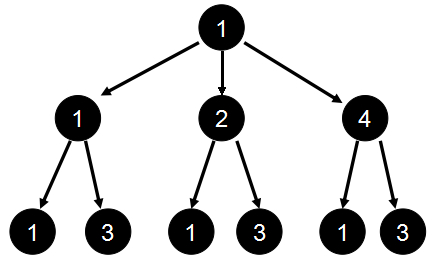
\includegraphics[height = 5cm,width = 9cm]{anti_prime.jpg}\\
这棵树除了第一层外,每一层对应着一个素数,从上到下递增;每一层的每一个节点对应着素数的幂,从左到右递增,每一条从根节点到叶节点的路径上数字相乘即为一个约数。 我们要想获得 $g(n)=x $的最小正整数,就要求$n$的质因子尽可能小,且尽可能多,换而言之就是幂次尽可能为$1$,所以就要对上面的树进行从上到下从左到右的$dfs$直到约数个数满足 $x$ 。 \\

\underline {【Codeforces 27E】给定一个数$n$,求一个最小的正整数,使得的约数个数为$n$.}

\begin{lstlisting}
typedef unsigned long long lint;
const lint inf = ~0ull;
const int prime[]= {2, 3, 5, 7, 11, 13, 17, 19, 23, 29, 31, 37, 41, 43, 47, 53};

int n;
lint ans;

void dfs(int depth, int limit, lint tmp, int num)
{
	if(num > n) return;
	if(num == n && tmp < ans) ans = tmp;
	for(int i = 1; i <= limit; ++i) { // i 相当于幂次
		if((double)tmp * prime[depth] > ans) break; // 不用扩展树的深度
		tmp *= prime[depth];
		if(n % (num * (i + 1)) == 0) {
			dfs(depth + 1, i, tmp, num * (i + 1));
		}
	}
}

int main()
{
	while(cin >> n){
		ans = inf;
		dfs(0, 63, 1, 1);
		cout << ans << endl;
	}
	return 0;
}
\end{lstlisting}

\underline {【URAL 1748】:给定一个数$n$,求$[1,n]$内约数个数最多的且数值最小的数,以及其约数个数$(n\leq 10^{18})$。}

\begin{lstlisting}
//将搜索改为当前值 tmp > n 时终止,初始化ans = inf, cnt = 0
//主函数里调用 dfs(0, 63, 1, 1) ,初始化 prime[] 同例1
void dfs(int depth, int limit, lint tmp, int num)
{
	if(tmp > n) return;
	if(num > cnt || (num == cnt && tmp < ans)) {
		ans = tmp;
		cnt = num;
	}
	for(int i = 1; i <= limit; ++i) {
		if((double)tmp * prime[depth] > n) break;
        //需要用 double 强制类型转换,否则爆数据
		tmp *= prime[depth];
		dfs(depth + 1, i, tmp, num * (i + 1));

	}
}
\end{lstlisting}

\section{卢卡斯定理}

用于解决组合数取模问题$C_{n}^{m}\ \% p\ \ (m\leq n \leq 10^{18},p$为素数) \\

当$1\leq m \leq n \leq 10^{18},2\leq p \leq 10^5$且$p$是素数时,如果: \\
$$n=n_kp^k+n_{k-1}p^{k-1}+...+n_1p+n_0$$
$$m=m_kp^k+m_{k-1}p^{k-1}+...+m_1p+m_0$$
那么: \\
$$C_{n}^{m}\ \% p=\prod_{i=0}^{k}C_{n_i}^{m_i}\ (mod \ p)$$
\begin{lstlisting}
inline ll C(ll a, ll b)
{ //计算组合数 C[a][b] ,如果是小数据并且模数固定可以预处理阶乘
	if(b > a) return 0;
	ll res = 1, x, y;
	for(int i = 1; i <= b; ++i) {
		x = (a + i - b) % mod;
		y = i % mod;
		res = res * x % mod * quick_pow(y, mod - 2) % mod; //模素数逆元
	}
	return res;
}
inline ll Lucas(ll n, ll m)
{
	if (n < 0 || m < 0 || m > n) return 0;
	if (m == 0) return 1;
	return C(n % mod, m % mod) * Lucas(n / mod, m / mod) % mod;
}
\end{lstlisting}

\subsection{给定$n$求$C_{n}^{m}(0\leq m\leq n\leq 10^8)$为奇数的$m$个数}

\underline {[HDU 4349]}

即$C_{n}^{m}\ \%2=1$的$m$个数,考虑将$n$和$m$都表示成$2$的幂次组合形式,则任意的系数$n_i$和$m_i$非0即1.因为$C_0^0=C_1^0=C_1^1=1$,所以根据$Lucas$定理,如果$n_i=0$,则$m_i=0$,如果$n_i=1$,则$m_i=0$或$1$,根据乘法原理每个$n_i=1$,对于$m_i$ 都有$2$种选择,那么$ans=2^{cnt}$,其中$cnt$ 是$n$分解为$2$的幂次形式系数为$1$的项个数

\begin{lstlisting}
scanf("%d", &n);
cnt = 0;
while (n) {
	if (n & 1) cnt ++;
	n >>= 1;
}
printf("%d\n", 1 << cnt);
\end{lstlisting}

\clearpage
\section{特殊方法}

\subsection{$n^k$的高三位}

对于给定的一个数$n$,它可以写成$10^a$,其中$a$为浮点数,则$n^k=(10^a)^k=10^{a*k}=10^x*10^y$;其中$x,y$分别是$a*k$的整数部分和小数部分.对于$t=n^k$这个数,它的位数由$10^x$决定,它的位数上的值则有$10^y$决定,因此我们要求$t$的前三位,只需要将$10^y$求出,在乘以$100$,就得到了它的前三位。$fmod(x,1)$可以求出$x$的小数部分。(或者使用$floor$函数)

\begin{lstlisting}
high_three_digits = (int)pow(10.0, 2.0 + fmod(k * 1.0 * log10(n * 1.0), 1)).
或者double t = 1.0 * k * log10(n * 1.0);
high_three_digits = (int)(pow(10.0, t - (int)floor(t) + 2.0));
\end{lstlisting}

\subsection{约数个数之和,定义$d(i)$为$i$的约数个数}

$$\sum_{i=1}^{a}d(i)=\sum_{}\lfloor {\frac{a}{i}}\rfloor$$
$$\sum_{i=1}^{a}\sum_{j=1}^{b}d(i*j)=\sum_{gcd(i,j)=1}\lfloor{\frac{a}{i}}\rfloor \lfloor{\frac{b}{j}}\rfloor$$
$$\sum_{i=1}^{a}\sum_{j=1}^{b}\sum_{k=1}^{c}d(i*j*k)=\sum_{gcd(i,j)=gcd(j,k)=gcd(i,k)=1}\lfloor{\frac{a}{i}}\rfloor \lfloor{\frac{b}{j}}\lfloor {\frac{c}{k}}\rfloor$$
这个性质可以推广到$n$维 \\

\underline {[BZOJ 3994]:求$\sum_{i=1}^{n}\sum_{j=1}^{m}d(i*j)$,定义$d(i)$为$i$的约数个数.$n,m\in [1, 50000]$}

$$\begin{aligned}
ans &=\sum_{gcd(i,j)=1}\lfloor{\frac{n}{i}}\rfloor \lfloor{\frac{m}{j}}\rfloor
&= \sum_{i=1}^{n}\lfloor{\frac{n}{i}}\rfloor\sum_{j=1}^{m} \lfloor{\frac{m}{j}}\rfloor
\end{aligned}$$

$定义g(n)=\sum_{i=1}^{n}\lfloor{\frac{n}{i}}\rfloor=\sum_{i= 1}^{n}d(i)$,只需要预处理出$g(n)$就可以在$O(\sqrt n)$时间范围内解决问题。如果选择分步加速的话,预处理的复杂度是$O(n\sqrt n)$,但是其实我们考虑每个数$i$的约数个数,然后$g(n)$就是前缀和了。\\
在线性筛时每个合数是被最小质因子筛掉的,我们只需要记录这个每个数$m$最小质因子的幂次$num[m],d[m]$记录$m$的约数个数,显然$d(m)$ 是积性函数.对于$m=i*prime[j]$,如果$i\ \% \  prime[j]!=0$,根据积性函数性质$num[m]=1,d[m]=d[i]*d[prime[j]],$否则$num[m]=num[i]+1,$ 因为$m$的约数个数是:$(e_1+1)*(e_2+1)*...*(e_k+1),e_i$ 是质因子分解后各质因子的幂次,我们考虑$m$从$i$的转移过程,$m$只比$i$在$prime[j]$的幂次上多$1$,所以$d[m]=\frac{d[i]}{num[i]+1]}*(num[i]+2)$.
\begin{lstlisting}
void GetMu()//线性时间预处理
{
	bs.set();
	prime_cnt = 0;
	mu[1] = d[1] = 1;
	for(int i = 2; i < MAX_N; ++i) {
		if(bs[i]) {
			prime[prime_cnt++] = i;
			mu[i] = -1;
			num[i] = 1;
			d[i] = 2;
		}
		for(int j = 0; j < prime_cnt && i * prime[j]  < MAX_N; ++j) {
			bs[i * prime[j]] = 0;
			if(i % prime[j]) {
				mu[i * prime[j]] = -mu[i];
				num[i * prime[j]] = 1;
				d[i * prime[j]] = d[i] * d[prime[j]];
			}else {
				mu[i * prime[j]] = 0;
				num[i * prime[j]] = num[i] + 1;
				d[i * prime[j]] = d[i] / (num[i] + 1) * (num[i] + 2);
				break;
			}
		}
	}
	for(int i = 1; i < MAX_N; ++i) {
		sum[i] = sum[i - 1] + mu[i];
		g[i] = g[i - 1] + d[i];
	}
}
void Get_g() // O(n * sqrt(n)) 的预处理
{
	int last;
	for(int n = 1; n < MAX_N; ++n) {
		for(int i = 1; i <= n; i = last + 1) {
			last = n / (n / i);
			g[n] += (ll) (last - i + 1) * (n / i);
		}
	}
}

inline ll solve(int n, int m)
{
	ll res = 0;
	int top = min(n, m), last;
	for(int i = 1; i <= top; i = last + 1) {
		last = min(n / (n / i), m / (m / i));
		res += (sum[last] - sum[i - 1]) * g[n / i] * g[m / i];
	}
	return res;
}
\end{lstlisting}

对于【Codeforces 235 E Number Challenge】:
$$\sum_{i=1}^{a}\sum_{j=1}^{b}\sum_{k=1}^{c}d(ijk),a,b,c\in [1,2000]$$
利用上述结论反演可得:
$$Ans =\sum_{i=1}^{i=a}{\lfloor{\frac{a}{i}}}\rfloor\sum_{d}^{min(b,c)}μ(d)\sum_{d|j,(i,j)=1}\lfloor{\frac{b}{j}}\rfloor\sum_{d|k,(i,k)=1}\lfloor{\frac{c}{k}}\rfloor$$
记$j=dj',k=dk'$,则:
$$Ans=\sum_{i=1}^{i=a}{\lfloor{\frac{a}{i}}}\rfloor\sum_{d}^{min(b,c)}μ(d)\sum_{gcd(i,dj')=1}\lfloor{\frac{b}{dj'}}\rfloor\sum_{gcd(i,dk')=1}\lfloor{\frac{c}{dk'}}\rfloor$$
因为$gcd(i,dj')=1$,我们先保证$gcd(i,d)=1,$然后枚举$j':1 \rightarrow \frac{b}{d}$,保证$gcd(i,j')=1$,这样就可以使得$gcd(i,dj')=1$,累加即可。对于$gcd(i,dk')=1$同样处理。时间复杂度是:$O(a*b*log(b))$

\begin{lstlisting}
//需要预处理 GetMu() 和 GetGcd()
inline ll work(int n, int x)
{
	ll res = 0;
	for(int i = 1; i <= n; ++i) {
		if(gcd[i][x] == 1) {
			res = (res + (n / i)) % mod;
		}
	}
	return res;
}

inline ll solve(int a, int b, int c)
{
	ll res = 0;
	int top = min(b, c);
	for(int i = 1; i <= a; ++i) {
		for(int d = 1; d <= top; ++d){
			if(gcd[i][d] == 1) {
				ll tmp = 0;
				tmp = (ll) (a / i) * mu[d] * work(b / d, i)
                            % mod * work(c / d, i) % mod;
				res = ((res + tmp) % mod + mod) % mod;
			}
		}
	}
	return res;
}
\end{lstlisting}

\subsection{给定$k$,求最小的$n$使得$n$的约数个数恰为$n-k$个$(k\leq 47777)$}
\underline {【HDU 4542】}

\begin{lstlisting}
const int MAX_N = 50010;
int id[MAX_N];
void init()
{
	for(int i = 1; i < MAX_N; ++i) id[i] = i;
// 初始化 id[i] 最多有 i 个数与其互质
	for(int i = 1; i < MAX_N; ++i) {
		for(int j = i; j < MAX_N; j += i) id[j]--;
//根据 j 的约数有 i,id[j]--
		if(id[id[i]] == 0) id[id[i]] = i;
		// 因为我们最终是要将 id[k] 表示成约数个数为 n-k 的最小数 n ,
        // 如果此时 id[id[i]]=0 说明小于 i 的数中不存在数 x , 使得 x 的约数个数为 x-id[i]
        // 那么实际上使得约数个数恰为 n-id[i] 的最小数 n 只能是 i 了
		id[i] = 0;
// 显然小于等于 i 的数不存在数 x 使得 x 的约数个数恰为 x-i 个,所以要赋 id[i]=0
	}
} // 对于 id[i] 等于 0 的 i ,实际上就不存在数 x 使得 x 的约数个数恰为 x-i 个
\end{lstlisting}

\subsection{$C_{n}^{m}\mod \ p(p=p_1*p_2$,且$p_1,p_2$为素数)}

我们把$C_{n}^{m}\ \ \% \ \ p$的值记为$x$,把$C_{n}^{m}\ \%\  p_1$的值记为$x1$,把$C_{n}^{m}\ \%\  p_2$的值记为$x2$,则有: \\
$$x \equiv \ x_1(\% \ \ p_1)\qquad x \equiv \ x_2(\% \ \ p_2)$$
因为$p_1,p_2$都是素数,所以$x_1$和$x_2$都可以用$Lucas$定理求解出来。利用中国剩余定理求解同余方程。\\
定义:
\begin{center}
$inv_1$为:($p_2$在模$p_1$域下的逆元)$*p_2$\\
$inv_2$为:($p_1$在模$p_2$域下的逆元)$*p_1$
\end{center}

\begin{lstlisting}
//quick_pow( a, b, c): (a ^ b) % c
inv1 = quick_pow(p2, p1 - 2, p1) * p2;
inv2 = quick_pow(p1, p2 - 2, p2) * p1;
\end{lstlisting}
那么答案就是:\\
$$x=(inv_1*x_1\ + inv_2 * x_2)\% \ p$$

%\end{document}
